\documentclass[11pt,titlepage,a4paper]{report}

%INCLUSIONE PACCHETTI
%---------------------------------------------
\usepackage[italian]{babel}
\usepackage{fancyhdr}
\usepackage{graphicx}
\graphicspath{{./pics/}} % cartella di salvataggio immagini

% STILE DI PAGINA
%---------------------------------------------
\pagestyle{fancy}
\renewcommand{\sectionmark}[1]{\markright{\thesection.\ #1}}
\lhead{\nouppercase{\rightmark}}
\rhead{\nouppercase{\leftmark}}
\renewcommand{\chaptermark}[1]{%
\markboth{\thechapter.\ #1}{}}

%Ridefinisco lo stile plain della pagina
\fancypagestyle{plain}{%
	\lhead{
\includegraphics[height=50pt]{logo.eps}}
	\chead{}
	\rhead{HappyCode inc \\ happycodeinc@gmail.com}
	\lfoot{BR-jsys}
	\rfoot{\dt - \lv}
	\cfoot{\thepage}
	\renewcommand{\headrulewidth}{1pt}
	\renewcommand{\footrulewidth}{1pt}
}

\begin{document}

%definizione variabili 
\newcommand{\lv}{ 0.3 } % latest version
\newcommand{\dt}{ Definizione del Prodotto }% Document title
\newcommand{\Glossario}{ Glossario.1.4.pdf }
%fine definizione variabili
\newcommand{\br}{business rule}
\newcommand{\brs}{business rules}
\newcommand{\bo}{business object}
\newcommand{\bos}{business objects}
\newcommand{\re}{repository}
\newcommand{\brp}{BusinessRuleParser}
\newcommand{\brl}{BusinessRuleLexer}
\newcommand{\BR}{BusinessRule}


\hyphenation{glos-sa-rio es-pli-ci-to ve-ri-fi-ca-re re-po-si-to-ry se-gna-la-ta coe-ren-za des-crit-te va-li-da-zio-ne ne-ces-sa-rio as-so-cia-zio-ne re-po-si-to-ry ri-chies-te de-scrit-te}
\begin{titlepage}\begin{center}
\vspace*{0.5in}

\includegraphics{logo.eps}
\vspace*{0.2in} \\
{\Large \textbf{BR-jsys}}
{\Large \emph{business rules} per sistemi gestionali in architettura J2EE } 
\vspace{2in} \\
\Huge \textsc{ \dt }
\par\rule{10cm}{0.4pt} \par {\large Versione \lv - \today} \\
\end{center}\end{titlepage}
\vspace*{0.5in}

\begin{center}
\thispagestyle{plain}
\begin{table}[htbp]
\large{
\begin{tabular}{l}
\Large{\textbf{\textsf{Capitolato: ''BR-jsys``}}} \\
\begin{tabular}{||p{6cm}||p{6cm}||}
\hline
\textbf{Data creazione:} & 18/11/2007 \\ \hline
\textbf{Versione:} & \lv \\ \hline
\textbf{Stato del documento:} & Formale, esterno \\ \hline
% ----------------------------------------------------------------------------autori
\textbf{Redazione:} & Carraro Filippo, Luca Appon \\ \hline
\textbf{Revisione:} & Michele Bortolato   \\ \hline
\textbf{Approvazione:}  & Luca Appon \\ \hline
\end{tabular} \\
\end{tabular}
}
\end{table}

\begin{table}[hbtp]
\large{
\begin{tabular}{l}
\Large{\textbf{\textsf{Lista di distribuzione}}} \\

\begin{tabular}{||p{6cm}||p{6cm}||} \hline
{HappyCode inc}& Gruppo di lavoro\\ \hline
{Tullio Vardanega, Renato Conte}& Rappresentanti del committente \\ \hline
{Zucchetti S.r.l}& Azienda committente\\ \hline
\end{tabular} \\
\end{tabular}
}
\end{table}
\begin{table}[hbtp]
\large{
\begin{tabular}{l}
\Large{\textbf{\textsf{Diario delle modifiche}}} \\
\begin{tabular}{||p{2cm}||p{3.5cm}||p{6cm}||} \hline
%-------------------------------------------------------------------------------diario modifiche
\textbf{Versione} & \textbf{Data rilascio} & \textbf{Descrizione} \\ \hline
0.3 & 05/02/2008 & Aggiunta del nome del file nel modello di documento\\ \hline
0.2 & 26/01/2008 & Documento sottoposto a revisionamento automatico\\ \hline
0.1 & 25/01/2008 & Stesura preliminare del documento \\ \hline

\end{tabular} \\
\end{tabular}

}
\end{table}
\end{center}
\newpage

\tableofcontents 

\chapter{Introduzione}
\section{Scopo del documento}
Il seguente documento ha lo scopo di descrivere l'architettura logica prodotta al termine della fase di progettazione architetturale. Descriver\`a in dettaglio i campi dati e i metodi appartenenti alle singole componenti del sistema ``BR-jsys''.
\section{Scopo del prodotto}
Per lo scopo del prodotto si faccia riferimento al documento ``Analisi dei Requisiti''.

\section{Glossario}
Viene fornito come documento esterno chiamato \Glossario.

\section{Riferimenti}
\begin{itemize}
\item Capitolato d'appalto concorso per sistema ``BR-jsys'';
\item Verbale dell'incontro con il committente ``Incontro2007-11-22.pdf'';
\item Verbale dell'incontro con il committente ``Incontro2008-02-05.pdf'';
\item ``Analisi dei Requisiti'';
\item ``Piano di Qualifica'';
\item ``Norme di Progetto'';
\item ``Specifica Tecnica'';
\item ``Ingegneria del Software'' 8a edizione - Ian Sommerville;
\item ``The Definitive ANTLR Reference'';
\item Manuale di eXist reperibile all'URL \textit{exist.sourceforge.net}.
\end{itemize}
\chapter{Standard di progetto}
\section{Standard di progettazione architetturale}
Per quanto riguarda le rappresentazioni grafiche dell'architettura del sistema ``BR-jsys'', ci siamo basati sulle regole definite da UML 2.1. In particolare, ci siamo appoggiati aull'uso di ``Poseidon for UML - professional edition 6.0.2''. Per i diagrammi use-cases ci siamo affidati invece a Dia 0.96.1.
\section{Standard di documentazione del codice}
Per le regole di documentazione del codice si faccia riferimento al documento ``Norme di Progetto'' allegato.
\section{Standard di denominazione di entit\`a e relazioni}
Per le regole di denominazione delle entit\`a, delle relazioni e degli oggetti, si faccia riferimento al documento ``Norme di Progetto'' allegato.
\section{Standard di programmazione}
Anche in questo caso, si faccia riferimento al documento ``Norme di Progetto'' allegato.
\section{Strumenti di lavoro}
L'azienda ha fatto uso dei seguenti strumenti di lavoro:
\begin{itemize}
\item Eclipse 3.3.1.1;
\item eXist 13.1.1.2; 
\item Latex 3.14;
\item ANTLRWorks 1.1.5.
\end{itemize}
\chapter{Specifica delle componenti}
\section{GUI}
\subsection{Diagramma delle classi}
\begin{center}
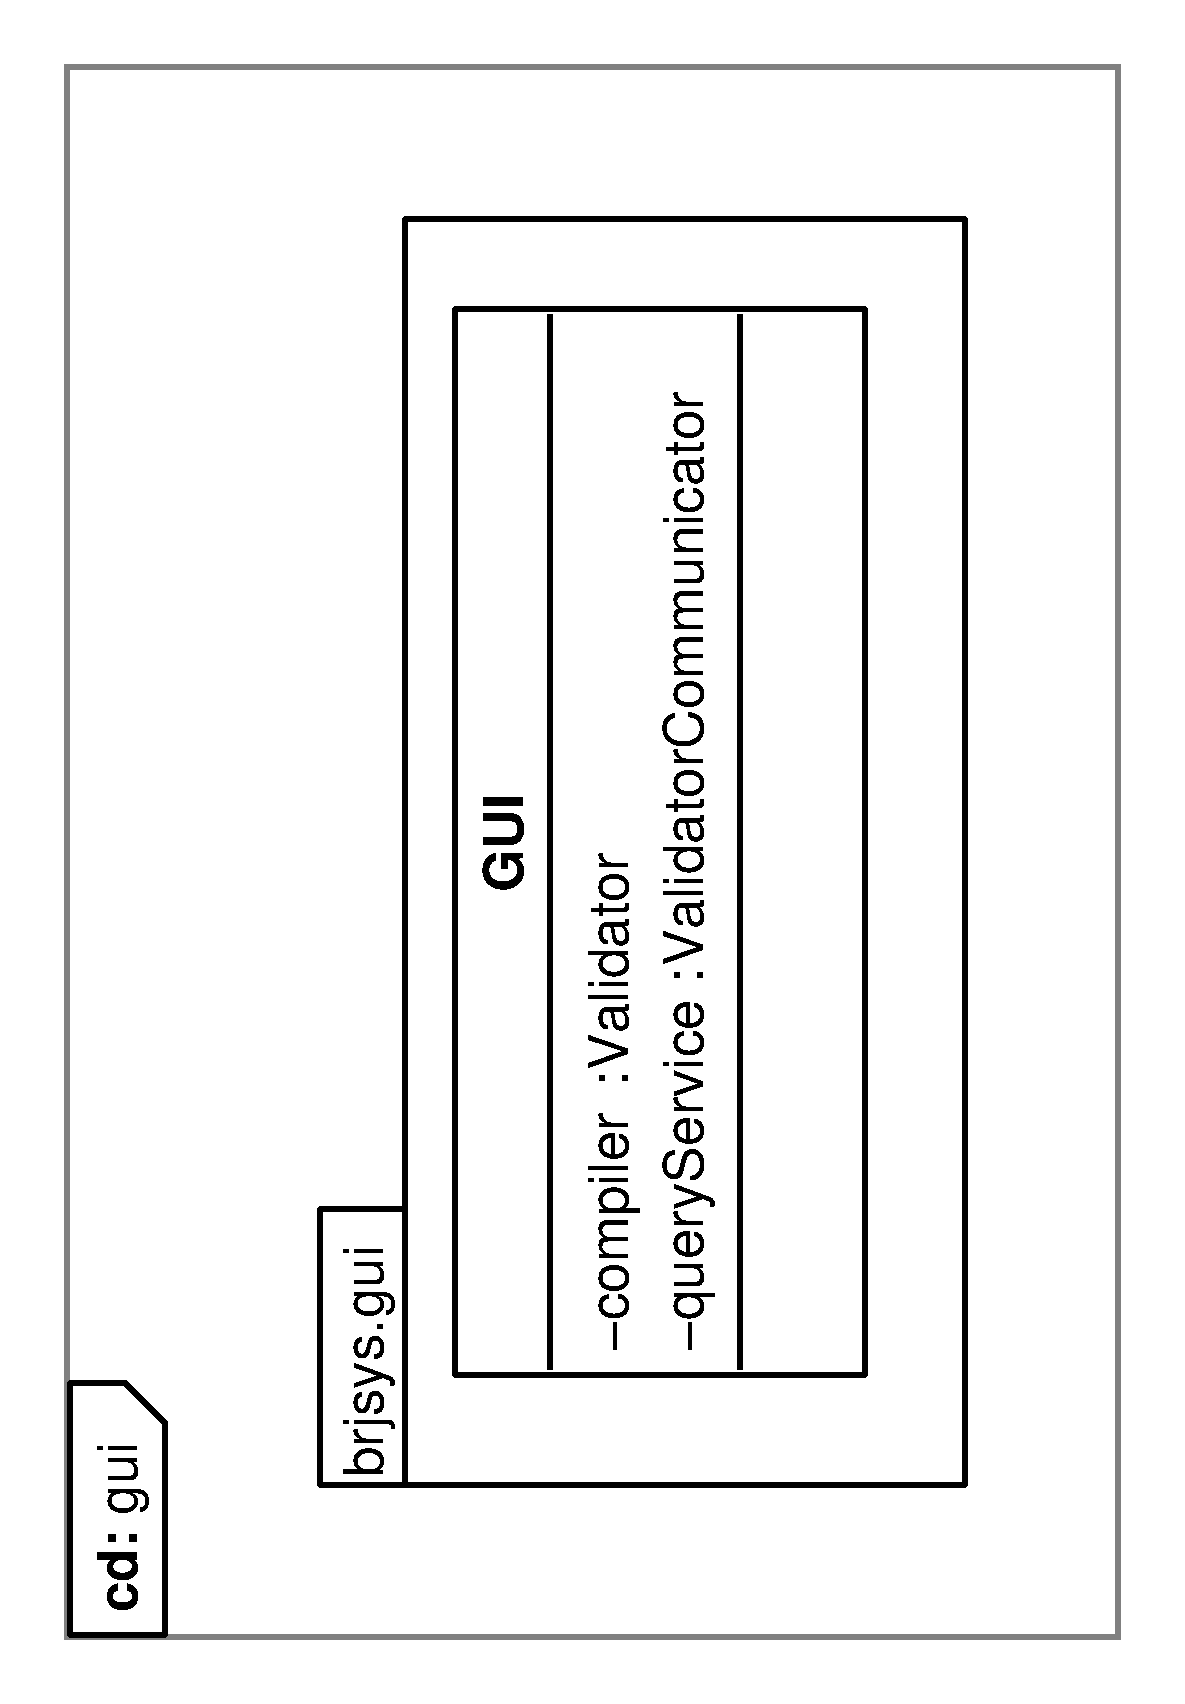
\includegraphics[width=0.3\textwidth, angle=-90]{DiagrammaClassi/gui.eps}
\end{center}
\subsection{Gui}
%Diagramma della classe GUI...comprensivo di package
\subsubsection{Tipo, obiettivo e funzione del componente}
Questa componente, realizzata tramite una singola classe java, fornisce all'utente un'interfaccia minimale che gli consente di effettuare operazioni di cancellazione e querying sul \re. Nel caso di esecuzione di una query definita dall'utente, verranno fornite anche informazioni relative ai tempi d'esecuzione.
\subsubsection{Relazioni d'uso di altre componenti}
Questa componente utilizza:
\begin{itemize}
 \item \BR\ per dichiarare una nuova \br\ da spedire al validatore;
 \item Validator per effettuare la validazione di una \br;
 \item GUICommunicator che tratteremo successivamente.
\end{itemize}
\subsubsection{Interfacce con e relazioni di uso da altre componenti}
Nessuna.
\subsubsection{Attivit\`a svolte e dati trattati}
Gui possiede i campi dato necessari per comunicare col validatore e col DBMS.
\begin{center}

\begin{tabular}{||p{6cm}||p{6cm}||} \hline
\hline
Attributo & Descrizione \\  \hline
-compiler: Validator & Rappresenta il validatore per le \br \\ \hline
-repository: GUICommunicator & Collega la componente al DBMS consentendogli di effettuare le Query.\\ \hline
\end{tabular}
\end{center}
\begin{center}
\begin{tabular}{||p{6cm}||p{6cm}||} \hline
\hline
Metodo & Descrizione \\  \hline
\underline{+main(args: String[]):Validator} & Metodo standard in java per l'avvio dell'applicazione. Si incaricher\`a di creare un oggetto Gui\\ \hline
+Gui() & Costruttore per Gui.\\ \hline
\end{tabular}
\end{center}


\section{Validatore}
\subsection{Diagramma delle classi}
\begin{center}
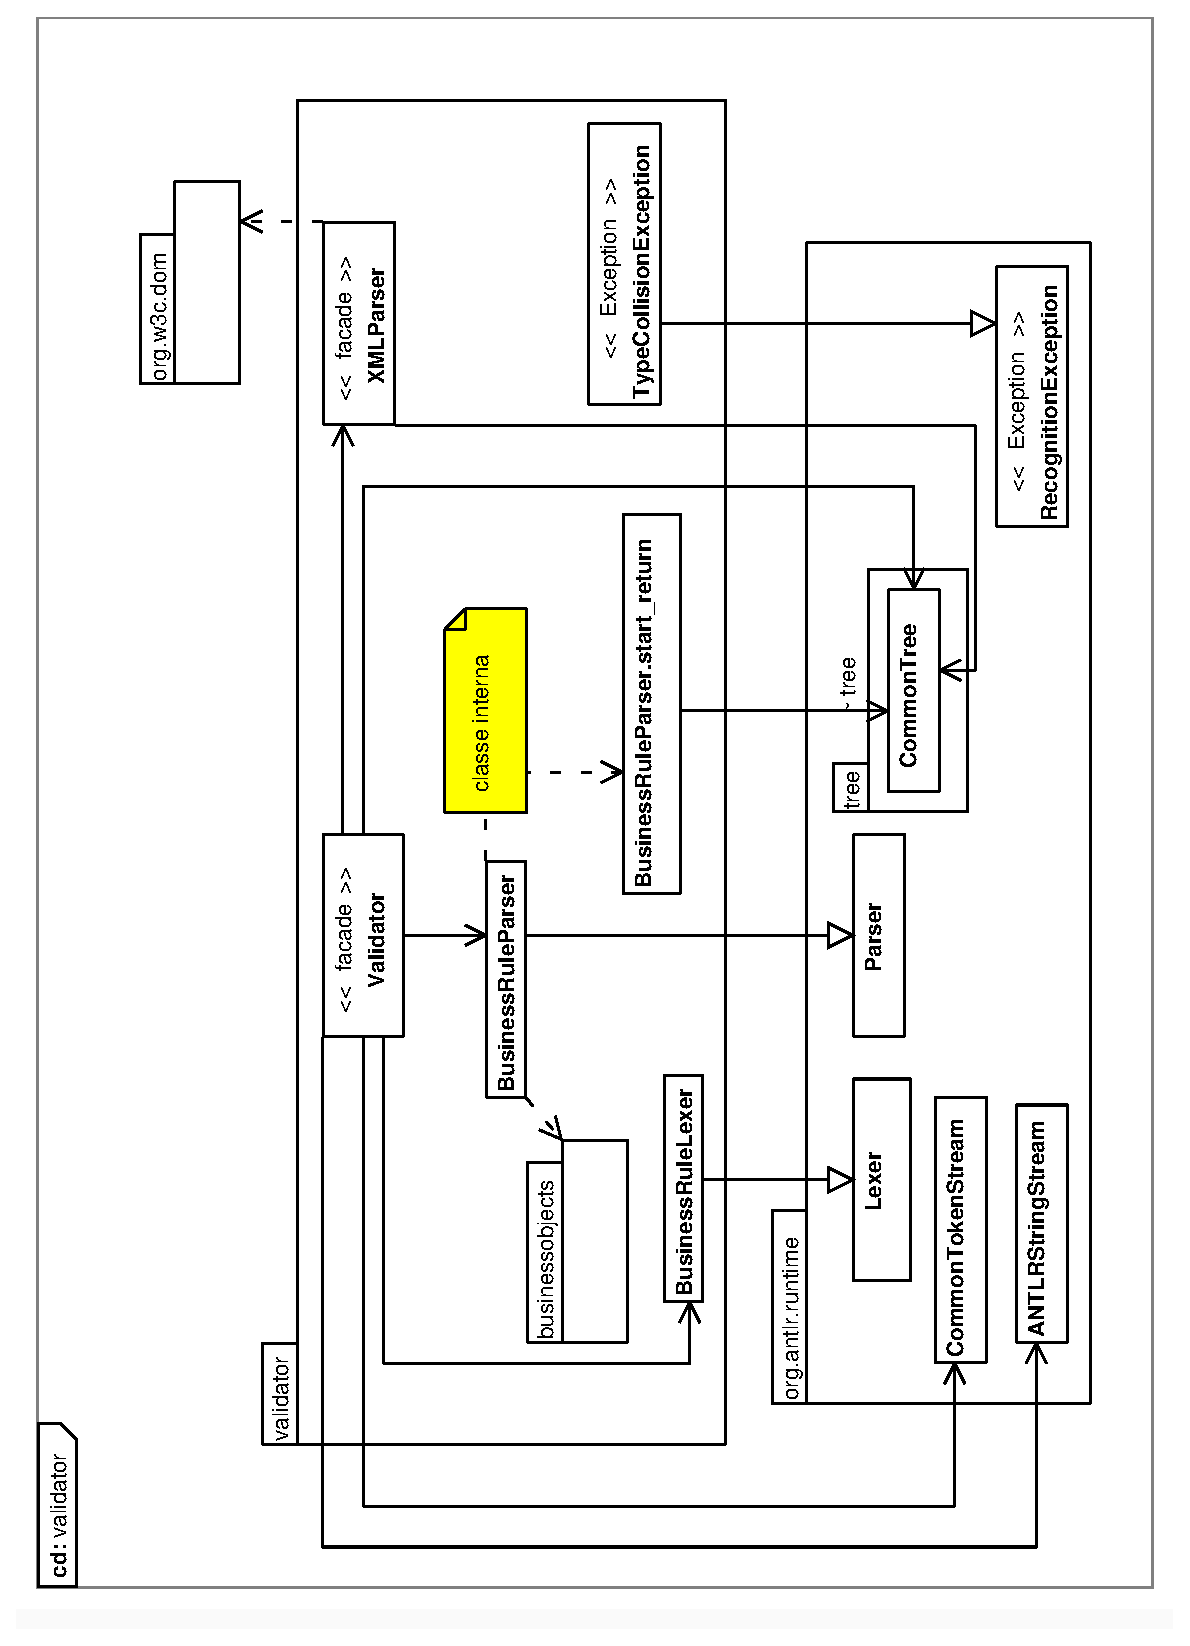
\includegraphics[width=0.6\textwidth, angle=-90]{DiagrammaClassi/validator.eps}
\end{center}
\subsection{Validator}%facade!!!->va descritto
\subsubsection{Tipo, obiettivo e funzione del componente}
La componente Validator effettua la validazione di una \br, dando la possibilit\`a all'utilizzatore di evitare le singole operazioni di compilazione. Ha il ruolo di \textit{fa\c{c}ade}: fornisce un'interfaccia unificata che riesce a gestire in maniera semplice ed immediata le operazioni di compilazione ed inserimento che avremmo altrimenti dovuto riportare direttamente laddove la componente GUI l'avrebbe richiesto.
\subsubsection{Relazioni d'uso di altre componenti}
Validator usa le componenti \brp, \brl, XMLParser e ValidatorCommunicator. Quest'ultime verranno ampliamente descritte in seguito.
\subsubsection{Interfacce con e relazioni di uso da altre componenti}
Validator \`e in relazione con la componente GUI, al fine di rendere possibile la validazione.
\subsubsection{Attivit\`a svolte e dati trattati}

\begin{center}
\begin{tabular}{||p{6cm}||p{6cm}||} \hline
\hline
Attributo & Descrizione \\  \hline
-repository: ValidatorCommunicator & Collega la componente al DBMS per inserire la \br\ validata nel \re.\\ \hline
\end{tabular}
\end{center}
\begin{center}
\begin{tabular}{||p{6cm}||p{6cm}||} \hline
\hline
Metodo & Descrizione \\  \hline
+Validator() & Costruttore di Validator.\\ \hline
+validate(rule: BusinessRule ): boolean \textbraceleft throws  RecognitionException \textbraceright& Unico metodo della componente che ricevuto in ingresso una \br\ ne effettua la validazione. Qualora si verificassero errori in fase di compilazione si restituir\`a un eccezione che verr\`a gestita dal chiamante. Se la \br\ viene inserita, il metodo ritorner\`a \textit{true}. Ritorner\`o invece \textit{false} se la regola ha un nome che \`e gi\`a presente nel \re.\\ \hline
\end{tabular}
\end{center}

\subsection{BusinessRuleLexer}
\subsubsection{Tipo, obiettivo e funzione del componente}
Questa componente, derivata da org.antlr.runtime.Lexer, non \`e altro che una classe wrapper per la stringa che rappresenta la \br. Essa aggiunge funzionalit\`a alla stringa, necessarie per il successivo parsing.
\subsubsection{Relazioni d'uso di altre componenti}
Nessuna.
\subsubsection{Interfacce con e relazioni di uso da altre componenti}
La componente BusinessRuleParser necessita della componente BusinessRuleLexer. Quest'ultima verr\`a approfondita successivamente.
\subsubsection{Attivit\`a svolte e dati trattati}
La componente, generata tramite un generatore di parser, dispone di numerosi campi dato per identificare i token della grammatica, nonch\`e vari metodi per la loro gestione. In definitiva si dovra\`a usare solo il suo costruttore.
\begin{center}
\begin{tabular}{||p{6cm}||p{6cm}||} \hline
\hline
Metodo & Descrizione \\  \hline
+BusinessRuleLexer(input: AntlrStringStream ) & Costruttore del componente.\\ \hline
\end{tabular}
\end{center}

\subsection{BusinessRuleParser}
\subsubsection{Tipo, obiettivo e funzione del componente}
Questa componente, derivata da org.antlr.runtime.Parser, effettua il parsing della stringa che rappresenta la \br. Effettua quindi il controllo sia sintattico che semantico della regola, facendo un ulteriore controllo sui tipi dei dati (siano essi costanti oppure campi dati di \bos). Mentre effettua la validazione, BusinessRuleParser genera l'albero di parsing secondo le specifiche presenti nel controllo semantico. \`E infine in grado di dare informazioni accurate riguardo eventuali errori in fase di validazione.
\subsubsection{Relazioni d'uso di altre componenti}
Questa componente necessita di un TokenStream, fornitogli indirettamente da BusinessRuleLexer. Deve riferirsi poi alla componente BusinessObjects per effettuare il controllo sui tipi per il \bo\ associato. Per trattare gli errori in fase di validazione ha bisogno invece della componente TypeCollisionException.
\subsubsection{Interfacce con e relazioni di uso da altre componenti}
\brp viene messa in relazione con XMLParser che verr\`a trattata successivamente.
\`E utilizzata inoltre dalla componente Validator.
\subsubsection{Attivit\`a svolte e dati trattati}
Questa componente, generata tramite un generatore automatico di parser, fornisce i campi dato per il riconoscimento dei token in appoggio a quelli gi\`a forniti dalla componente \brp. Contiene vari metodi privati per il controllo sintattico e semantico, per il parsing e contiene infine classi innestate incaricate di generare l'AST.
\begin{center}
\begin{tabular}{||p{6cm}||p{6cm}||} \hline
\hline
Attributo & Descrizione \\  \hline
+endParsing: BusinessRuleParser.start\_return & Campo dati che contiene l'AST da convertire in XML.\\ \hline 
\end{tabular}
\end{center}
\begin{center}
 \begin{tabular}{||p{6cm}||p{6cm}||}\hline
Metodo & Descrizione \\  \hline
+BusinessRuleParser(input: CommonTokenStream, associated: String) & Costruttore della componente. Il primo parametro identifica lo stream generato nelle fasi precedenti, il secondo dice qual'\`e il \bo\ associato alla regola.\\ \hline
+start(): BusinessRuleParser.start\_return \textbraceleft throws\phantom{c}RecognitionException \textbraceright & Risultato del parsing corretto di una \br. Contiene al suo interno l'AST. Nel caso di errore nella validazione il chiamante dovr\`a gestire opportunamente l'eccezione.\\ \hline
\end{tabular}
\end{center}


\subsection{TypeCollisionException}
\subsubsection{Tipo, obiettivo e funzione del componente}
Questa componente, derivata dalla classe org.antlr.runtime.RecognitionException, permette di ricavare informazioni sugli eventuali errori avvenuti in fase di parsing della \br. In definitiva aggiunge alla sua superclasse la possibilit\`a di riportare informazioni su errori di tipo.
\subsubsection{Relazioni d'uso di altre componenti}
Nessuna.
\subsubsection{Interfacce con e relazioni di uso da altre componenti}
La componente TypeCollisionException \`e utilizzata da \brp\ per sollevare eccezioni derivanti da errori di tipo.
\subsubsection{Attivit\`a svolte e dati trattati}
Viene ridefinito il metodo printStackTrace() e messo a disposizione un costruttore per avere informazioni sui tipi che si sono rivelati incompatibili.
\begin{center}
\begin{tabular}{||p{6cm}||p{6cm}||} \hline
\hline
Attributo & Descrizione \\  \hline
-first:Class & Identifica il tipo del primo elemento che ha causato un'operazione incompatibile. \\ \hline
-second:Class & Identifica il tipo del secondo elemento che ha causato un'operazione incompatibile \\ \hline
\end{tabular}
\end{center}
\begin{center}
\begin{tabular}{||p{6cm}||p{6cm}||} \hline
\hline
Metodo & Descrizione \\  \hline
+TypeCollisionException(typeA: Class, typeB: Class ) & Costruttore a due parametri che rappresentano i due tipi che sono entrati in conflitto.\\ \hline
+printStackTrace() & Metodo ridefinito che consente di visualizzare correttamente la struttura dell'errore avvenuto.\\ \hline
\end{tabular}
\end{center}

\subsection{XMLParser}%probabilmente è un facade anche questo
\subsubsection{Tipo, obiettivo e funzione del componente}
La componente XMLParser si occupa di effettuare la conversione dell'albero sintattico prodotto dalla componente \brp\ in un elemento XML rappresentante la \br. L'elemento XML risultante conterr\`a:
\begin{itemize}
 \item il nome della \br, che dovr\`a essere univoco;
 \item il nome del \bo\ associato alla regola;
 \item la struttura dell'AST della \br, scritta secondo la metodologia elemento-attributo tipica di XML;
 \item la struttura dell'AST della \br, scritta linearmente secondo la notazione prefissa rappresentata da un singolo attributo XML;
 \item la \br\ effettivamente digitata dall'utente;
 \item eventuali commenti associati dall'utente alla \br.
\end{itemize}
XMLParser ha in questo contesto il ruolo del design pattern \textit{fa\c{c}ade}. La creazione di un elemento XML tramite il package java \textit{org.w3c.dom} necessita di operazioni sequenziali che coinvolgono numerose classi e numerosi metodi. Implementare tutte queste procedure direttamente nella classe Validator renderebbe il codice meno leggibile e meno manipolabile.
\subsubsection{Relazioni d'uso di altre componenti}
XMLParser ha bisogno dell'AST prodotto da \brp, nonch\`e necessita della componente \br\ per ricavare le informazioni da inserire nell'elemento XML.
\subsubsection{Interfacce con e relazioni di uso da altre componenti}
La componente ValidatorCommunicator ha bisogno dell'elemento XML prodotto da XMLParser per avviare la procedura di inserimento nel \re.
\subsubsection{Attivit\`a svolte e dati trattati}
XMLParser contiene le operazioni per scorrere l'AST ed effettuare la traduzione in XML. Dispone inoltre di una tabella Hash statica che serve per associare i valori numerici che il parser usa per identificare i token ai nomi dei tokens definiti dall'utente.
\begin{center}
\begin{tabular}{||p{6cm}||p{6cm}||} \hline
\hline
Attributo & Descrizione \\  \hline
\underline{-simbols:}\underline{HashTable\textless Integer,String\textgreater}& Nell'AST il tipo di token viene rappresentato tramite un numero univoco. Per poter associare in maniera rapida i tokens ai numeri che li rappresentano \`e dunque necessario generare una tabella Hash. Le informazioni riguardo l'associazione sono riportate in un file di nome \textit{BusinessRule.tokens} generato automaticamente dal generatore di parser.\\ \hline
\end{tabular}
\end{center}
\begin{center}
\begin{tabular}{||p{6cm}||p{6cm}||} \hline
\hline
Metodo & Descrizione \\  \hline
\underline{-generateSimbols():} \underline{HashTable\textless Integer, String \textgreater} & Questo metodo legge il file \textit{BusinessRule.tokens} dal quale ricava tutte le associazioni tra il numero associato al token e la stringa che gli si associa in fase di costruzione dell'attributo \textit{simbols}.\\ \hline
+parse(AST: Tree, rule: BusinessRule): String & Metodo pubblico che si incarica di effettuare la conversione da AST a stringa che rappresenta l'elemento XML. Si dovr\`a seguire la procedura adeguata per la creazione di un elemento strutturato XML secondo le specifiche delle librerie \textit{org.w3c.dom}\\ \hline
-scanAST(AST: Tree, root: Element, doc: Document) Element & Metodo privato che scorre ricorsivamente l'AST per convertirla in un elemento XML. La regola verr\`a successivamente inserita nel \re. \\ \hline
\end{tabular}
\end{center}

\subsection{businessobjects}%è un package
\subsubsection{Tipo, obiettivo e funzione del componente}
La componente businessobjects si occupa di offrire un namespace comune a tutti i \bos\ che durante la validazione di una \br\ vengono interpellati richiedendo accesso ai suoi campi o sottocampi.
\subsubsection{Relazioni d'uso di altre componenti}
Nessuna.
\subsubsection{Interfacce con e relazioni di uso da altre componenti}
\brp\ necessita di questa componente per effettuare il controllo dei tipi qualora fosse necessario.
\subsubsection{Attivit\`a svolte e dati trattati}
Il componente businessobjects offre le classi java che rappresentano i \bos.

\section{Business Rule}
\subsection{Diagramma delle classi}
\begin{center}
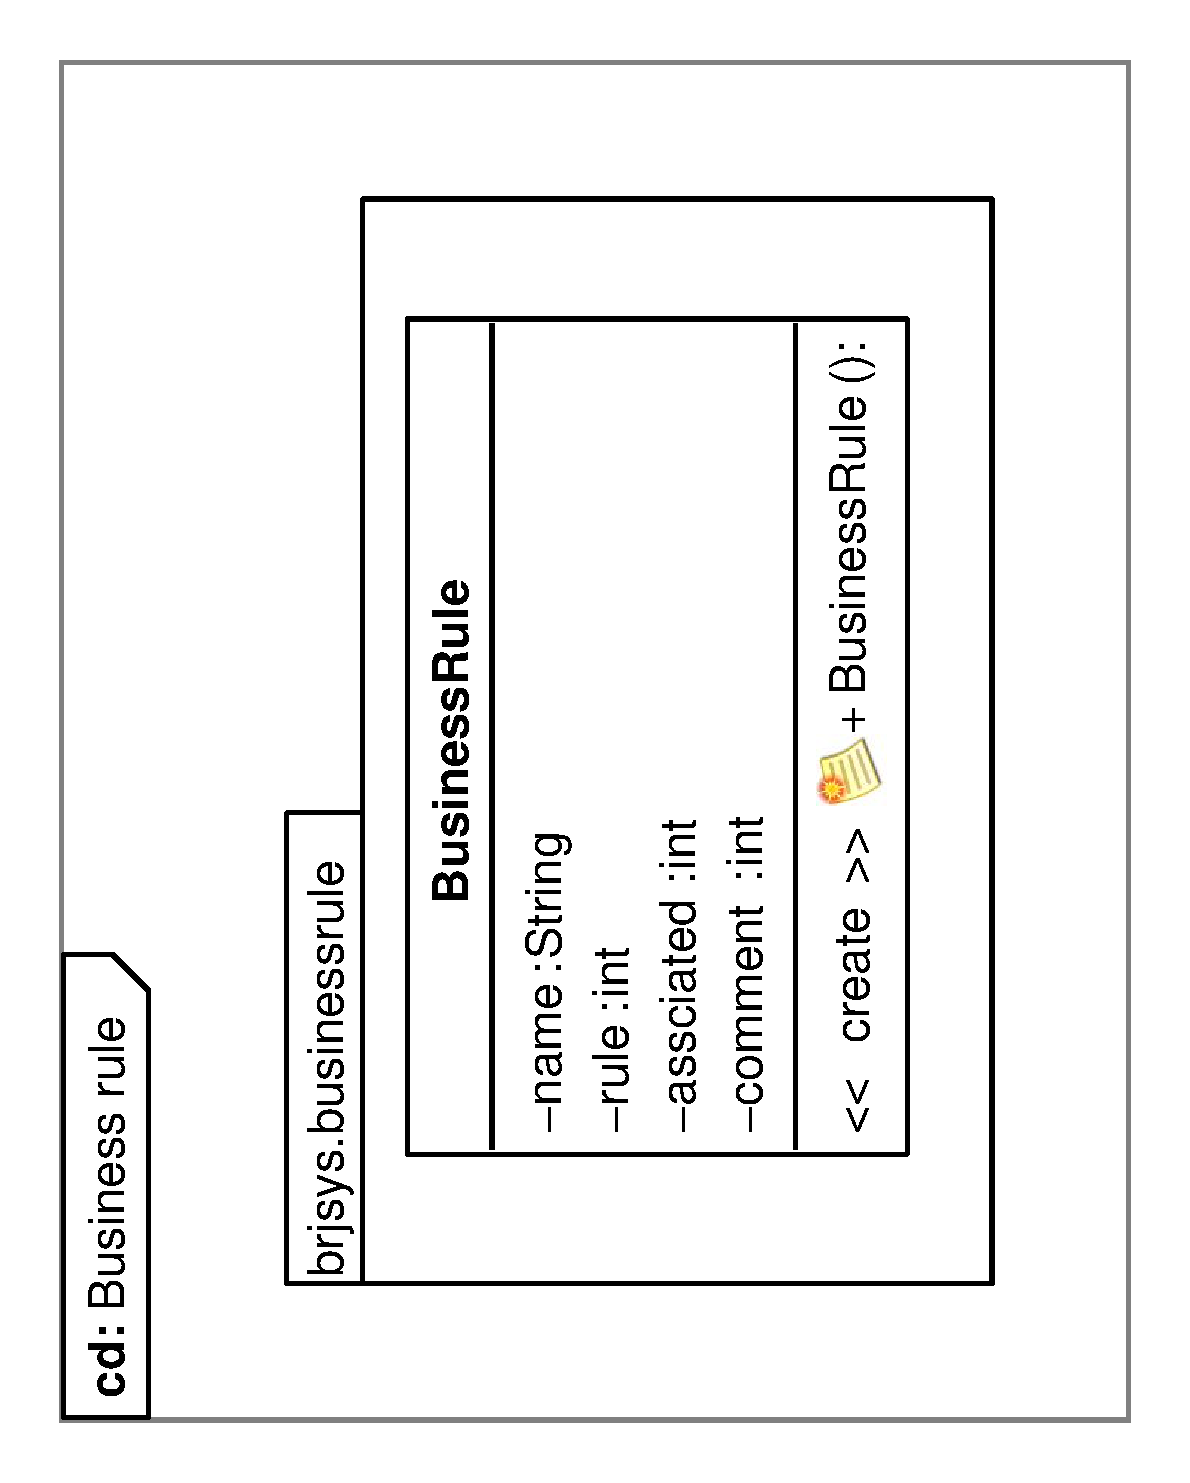
\includegraphics[width=0.3\textwidth, angle=-90]{DiagrammaClassi/Businessrule.eps}
\end{center}
\subsection{BusinessRule}
\subsubsection{Tipo, obiettivo e funzione del componente}
La componente \BR\ rappresenta la \br\ che l'utente inserisce e vuole validare.
\subsubsection{Relazioni d'uso di altre componenti}
Nessuna.
\subsubsection{Interfacce con e relazioni di uso da altre componenti}
La componente GUI utilizza \BR\ nel caso in cui l'utente voglia inserire una nuova \br.
La componente Validator effettua la validazione di un'istanza di \BR, tramite la chiamata del suo metodo validate().
\subsubsection{Attivit\`a svolte e dati trattati}
La componente contiene i campi dato Stringa per rappresentare una business rule ossia name, associatedObject, rule e comment, quest'ultima pu\'o non essere istanziata, vengono inoltre messi a disposizione il costruttore e il metodo ridefinito toString().
\begin{center}
\begin{tabular}{||p{6cm}||p{6cm}||} \hline
\hline
Attributo & Descrizione \\  \hline
+name:String &  Denota il nome della \br.\\ \hline
+associated:String & Denota il \bo\ assocato.\\ \hline
+rule:String &  Denota la \br\ scritta dall'utente e da validare.\\ \hline
+comment:String & Denota un commento opzionale che l'utente pu\`o associare a quella \br.\\ \hline
\end{tabular}
\end{center}
\begin{center}
\begin{tabular}{||p{6cm}||p{6cm}||} \hline
\hline
Metodo & Descrizione \\  \hline
BusinessRule(nameR: String , associatedR: String, ruleR: String, commentR: String) & Costruttore di BusinessRule.\\ \hline
\end{tabular}
\end{center}

\section{Comunicatore}
\subsection{Diagramma delle classi}
\begin{center}
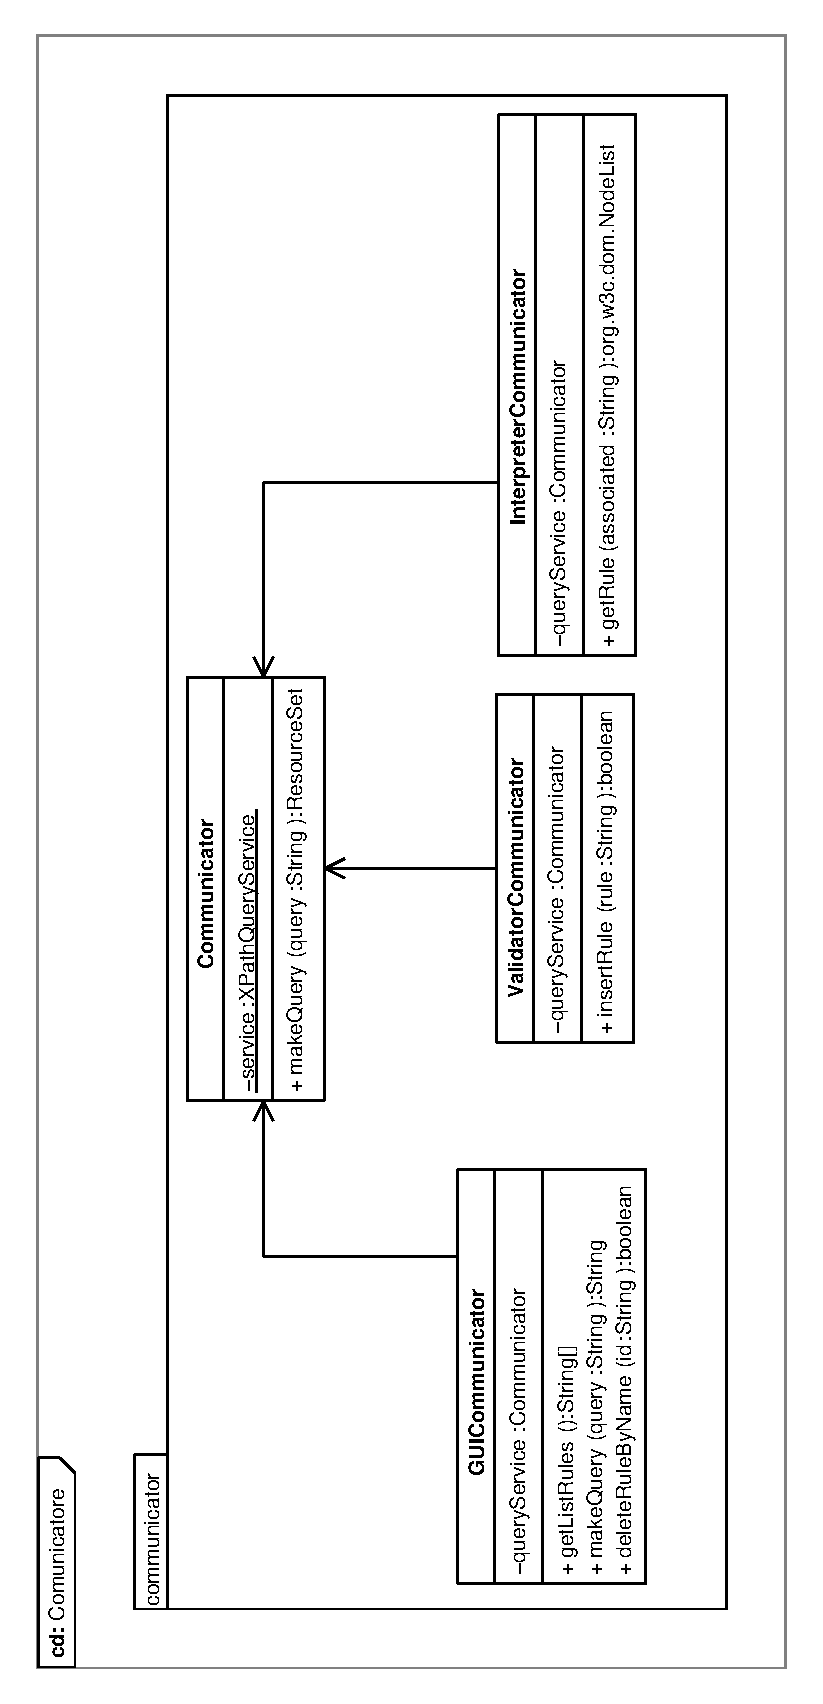
\includegraphics[width=0.5\textwidth, angle=-90]{DiagrammaClassi/Comunicatore.eps}
\end{center}
Durante la fase di progettazione la Happycode ha fatto diversi studi sui DBMS in grado di trattare basi di dati XML. Si \`e infine presa la decisione di adottare eXist in quanto oltre ad essere stato consigliato dal proponente, si \`e rivelato il pi\`u adatto alle nostre esigenze. EXist oltre a garantire buone prestazioni, mette a disposizione pi\`u funzionalit\`a rispetto ai suoi concorrenti e consente di sviluppare applicazioni java che si interfacciano al DBMS stesso.
\subsection{Communicator}
\subsubsection{Tipo, obiettivo e funzione del componente}
Communicator fornisce alle componenti che la utilizzano la possibilit\`a di effettuare query di qualsiasi tipo al \re\ presente nel DBMS.
\subsubsection{Relazioni d'uso di altre componenti}
Communicator necessita di interagire con la componente esterna DBMS per interrogare il \re.
\subsubsection{Interfacce con e relazioni di uso da altre componenti}
Le componenti GUICommunicator, InterpreterCommunicator e ValidatorCommunicator necessitano di Communicator per potergli passare Query specifiche. Le loro descrizioni verranno trattate successivamente.
\subsubsection{Attivit\`a svolte e dati trattati}
Quando viene istanziata per la prima volta inizializza la connessione al DBMS tramite la definizione di una variabile statica che successivamente consente di interrogare il \re direttamente passandogli la stringa che rappresenta la query composta secondo le specifiche XQuery.
\begin{center}
\begin{tabular}{||p{6cm}||p{6cm}||} \hline
\hline
Attributo & Descrizione \\  \hline
\underline{-service:XPathQueryService} & Consente, se istanziato correttamente, di comunicare con risorse presenti su eXist, in particolare faremo in modo configurarlo in modo che faccia query solamente nel \re posizionato in una posizione specifica nel DBMS.\\ \hline
-correctUsername:String & Memorizza il corretto username utilizzato per l'accesso.\\ \hline
-correctPassword:String & memorizza la corretta password utilizzata per l'accesso.\\ \hline
\end{tabular}
\end{center}
\begin{center}
\begin{tabular}{||p{6cm}||p{6cm}||} \hline
\hline
Metodo & Descrizione \\  \hline
+Communicator(username: String, password: String) & Costruttore di Communicator. Nel caso si acceda alla classe per la prima volta durante l'esecuzione del programma si istanzierà l'attributo service, se la connessione \`e andata a buon fine gli attributi correctUsername e correctPassword verranno settati con i valori corrispondenti.Altrimeti se l'attributo service \`e gi\`a stato istanziato non si far\`a altro che assicurarsi che i parametri in ingresso al costruttore corrispondano a quelli presenti negli attributi.\\ \hline
+makeQuery(query:String) :ResourceSet & Metodo pubblico che ricevuto in ingresso una query scritta secondo le specifiche XQuery la esegue e ne restituisce il risultato.Si dovr\`a gestire il caso di query mal formata. \\\hline
\end{tabular}
\end{center}

\subsection{GUICommunicator}
\subsubsection{Tipo, obiettivo e funzione del componente}
La componente contiene metodi necessari per modellare query di cancellazione (tramite operazioni XQuery Update) e query di semplice interrogazione.
\subsubsection{Relazioni d'uso di altre componenti}
GUICommunicator utilizza la componente Communicator per accedere al \re\ ed interrogarlo.
\subsubsection{Interfacce con e relazioni di uso da altre componenti}
GUICommunicator viene messa in relazione con la componente GUI, dalla quale riceve richieste di cancellazione e di querying.
\subsubsection{Attivit\`a svolte e dati trattati}
GUICommunicator sar\`a strutturata nel seguente modo:
\begin{center}
\begin{tabular}{||p{6cm}||p{6cm}||} \hline
\hline
Attributo & Descrizione \\  \hline
-queryService:Communicator & Permette alla componente di colloquiare con eXist.\\ \hline
\end{tabular}
\end{center}
\begin{center}
\begin{tabular}{||p{6cm}||p{6cm}||} \hline
\hline
Metodo & Descrizione \\  \hline
+GUICommunicator(username: String, password: String) & Costruttore del componente, username e password saranno utilizzati per l'istanziazione di queryService. \\ \hline

+deleteRuleByName(id: String): boolean & Metodo per Cancellare un \br\ dato il suo identificativo, se la \br\ è stata trovata nel \re\ e dunque cancellata ritorner\`a \textit{true} altrimenti \textit{false}.\\ \hline

+makeQuery(query: String):String & Metodo per eseguire una query in XQuery, dovr\`o fare attenzione che la struttura della query non contenga istruzioni XQuery Update che permetterebbero all'utente di modificare a piacimento il \re\ rendendolo inconsistente.\\ \hline

+getListRules(): String[]& Metodo che ritorna informazioni riguardo le query scritte nel \re. in particolare l'array di ritorno avr\`a un elemento per \br nel \re ed ogni elemento conterr\`a il nome, la regola, il \bo associato e l'eventuale commento.\\ \hline
\end{tabular}
\end{center}

\subsection{InterpreterCommunicator}
\subsubsection{Tipo, obiettivo e funzione del componente}
InterpreterCommunicator contiene metodi necessari per rispondere a richieste di \br\ da parte di un interprete esterno.
\subsubsection{Relazioni d'uso di altre componenti}
InterpreterCommunicator utilizza la componente Communicator per accedere al \re\ ed interrogarlo.
\subsubsection{Interfacce con e relazioni di uso da altre componenti}
La componente InterpreterCommunicator viene messa in relazione con l'interprete esterno, dal quale riceve richieste di \brs associate ad un determinato \bo.
\subsubsection{Attivit\`a svolte e dati trattati}
InterpreterCommunicator offre il metodo getRule() per richiedere le \br associate al \bo.

\begin{center}
\begin{tabular}{||p{6cm}||p{6cm}||} \hline
\hline
Attributo & Descrizione \\  \hline
-queryService:Communicator & Permette alla componente di colloquiare con eXist.\\ \hline
\end{tabular}
\end{center}
\begin{center}

\begin{tabular}{||p{6cm}||p{6cm}||} \hline
\hline
Metodo & Descrizione \\  \hline
+InterpreterCommunicator( username: String, password: String) & Costuttore con funzionamento analogo a GUICommunicator.\\ \hline
+getRule(associated: String): NodeList & Dato in input un \bo ritorna tutte le \brs che sono associate ad esso. \\ \hline
\end{tabular}
\end{center}

\subsection{ValidatorCommunicator}
\subsubsection{Tipo, obiettivo e funzione del componente}
ValidatorCommunicator contiene metodi necessari per effettuare l'inserimento di una \br\ validata gi\`a tradotta in XML.
\subsubsection{Relazioni d'uso di altre componenti}
ValidatorCommunicator utilizza la componente Communicator per accedere al \re\ ed interrogarlo.
\subsubsection{Interfacce con e relazioni di uso da altre componenti}
ValidatorCommunicator viene messa in relazione con la componente Validator per effettuare l'inserimento.
\subsubsection{Attivit\`a svolte e dati trattati}
ValidatorCommunicator offre il metodi insertRule() per inserire la \br\ nel \re. L'inserimento avverr\`a soltanto se la \br\ ha un nome che non \`e ancora presente nel \re.
\begin{center}
\begin{tabular}{||p{6cm}||p{6cm}||} \hline
\hline
Attributo & Descrizione \\  \hline
-queryService:Communicator & Permette alla componente di colloquiare con eXist.\\ \hline
\end{tabular}
\end{center}
\begin{center}
\begin{tabular}{||p{6cm}||p{6cm}||} \hline
\hline
Metodo & Descrizione \\  \hline
ValidatorCommunicator(username: String, password: String) & Costruttore con comportamento analogo a GUICommunicator.\\ \hline
insertRule(rule: String, idRule: String): boolean & Inserisce la \br\ nel \re\ soltanto se il suo nome non \`e gi\`a presente. Se l'inserimento \`e andato a buon fine ritorner\`a \textit{true}.\\ \hline
\end{tabular}
\end{center}

\chapter{Appendice}
\section{Tracciamento relazione componenti - requisiti}

\begin{tabular}{||p{4.8cm}||p{5.3cm}||p{3.9cm}||}\hline
\hline
Componente & Metodo Associato & Requisiti \\\hline
Gui & +Gui() & F4, F5, F7, F8 \\\cline{2-3}
& +main(args:String[]) & \bigskip \\\hline

Validator & +Validator() & F2, F5, F8 \\\cline{2-3}
& +validate() & F2, F3, F4, F5, F8, Npr1, NQ1 \\\hline

BusinessRuleLexer & +BusinessRuleLexer() & F2, F4, NQ1 \\\hline

BusinessRuleParser & BusinessRuleParser() & F2, F4, F10 \\\cline{2-3}
& +start() & F2, F4, F10, NQ1 \\\hline

TypeCollisionException & +TypeCollisionException() & F2, F4, F10, NQ1 \\\cline{2-3}
& +printStackTrace() & F2, F4, F10 \\\hline

XMLParser & -generateSimbols() & NPo1 \\\cline{2-3}
& +parse() & NPo1 \\\cline{2-3}
& -scanAST() & NPo1 \\\hline

businessobject & \bigskip & F2, F10, F11 \\\hline

BusinessRule & +BusinessRule() & F2, F10, F11, NU1, NU2, NU3, NQ1 \\\hline

Communicator & +Communicator() & F3, F5, F6, NPr1 \\\cline{2-3}
& +makeQuery() & F3, F5, F6, NPr1 \\\hline

GUICommunicator & +GUICommunicator() & F5, F7, F8 \\\cline{2-3}
& +deleteRuleByName() & F5, F7, F8 \\\cline{2-3}
& +makeQuery() & F5, F8 \\\cline{2-3}
& +getListRules() & F5, F8 \\\hline

InterpreterCommunicator & +InterpreterCommunicator() & F5, F6 \\\cline{2-3}
& +getRule() & F5, F6 \\\hline

ValidatorCommunicator & +ValidatorCommunicator() & F3 \\\cline{2-3}
& +insertRule() & F3 \\\hline
\end{tabular}

\newpage

\end{document}
